\chapter{Proposed Solution}

%As stated by Sadana et al. \cite{sadana_redefining_2016}, it is also important to explore how existing techniques can be applied to new platforms like virtual reality devices.
%We got inspired by a circular form of a tree map plot for hierarchical structures (see Figure \ref{fig:hierarchicalCirclePlot}). Each node can either be a simple leaf node or a network itself. So we need a way to visualize connections between different networks, a way to do this is a multilayer network visualization see Figure \ref{fig:2dmultilayerVis}. Here each flat layer represents a different network but a hierarchical relationship is not always given for these visualizations.  
\section{Initial Problem}

The idea to build our own visualization began as we wanted to improve the original visualization of the comorbidity network we saw in Figure \ref{fig:original2DdiseaseNet}. Data analysts use this and similar datasets to discover possible coherences, correlations, distributions, clusters and more in the data. 
However, the visualization was not optimal because it hides links and first and foremost is limited to only one hierarchical layer. This is not a problem for this dataset in particular, but we wanted a solution to visualize n hierarchical networks.\\
Therefore, our goal is to develop a new visualization tool which supports data analysts in their daily work analyzing hierarchical networks, with the comorbidity network as a first real world data example. To test the usability of the visualization for n hierarchical networks we created some randomized networks as test data. 

\section{Main concept}

\subsection{Layout}

\begin{figure}[h]
    \centering
    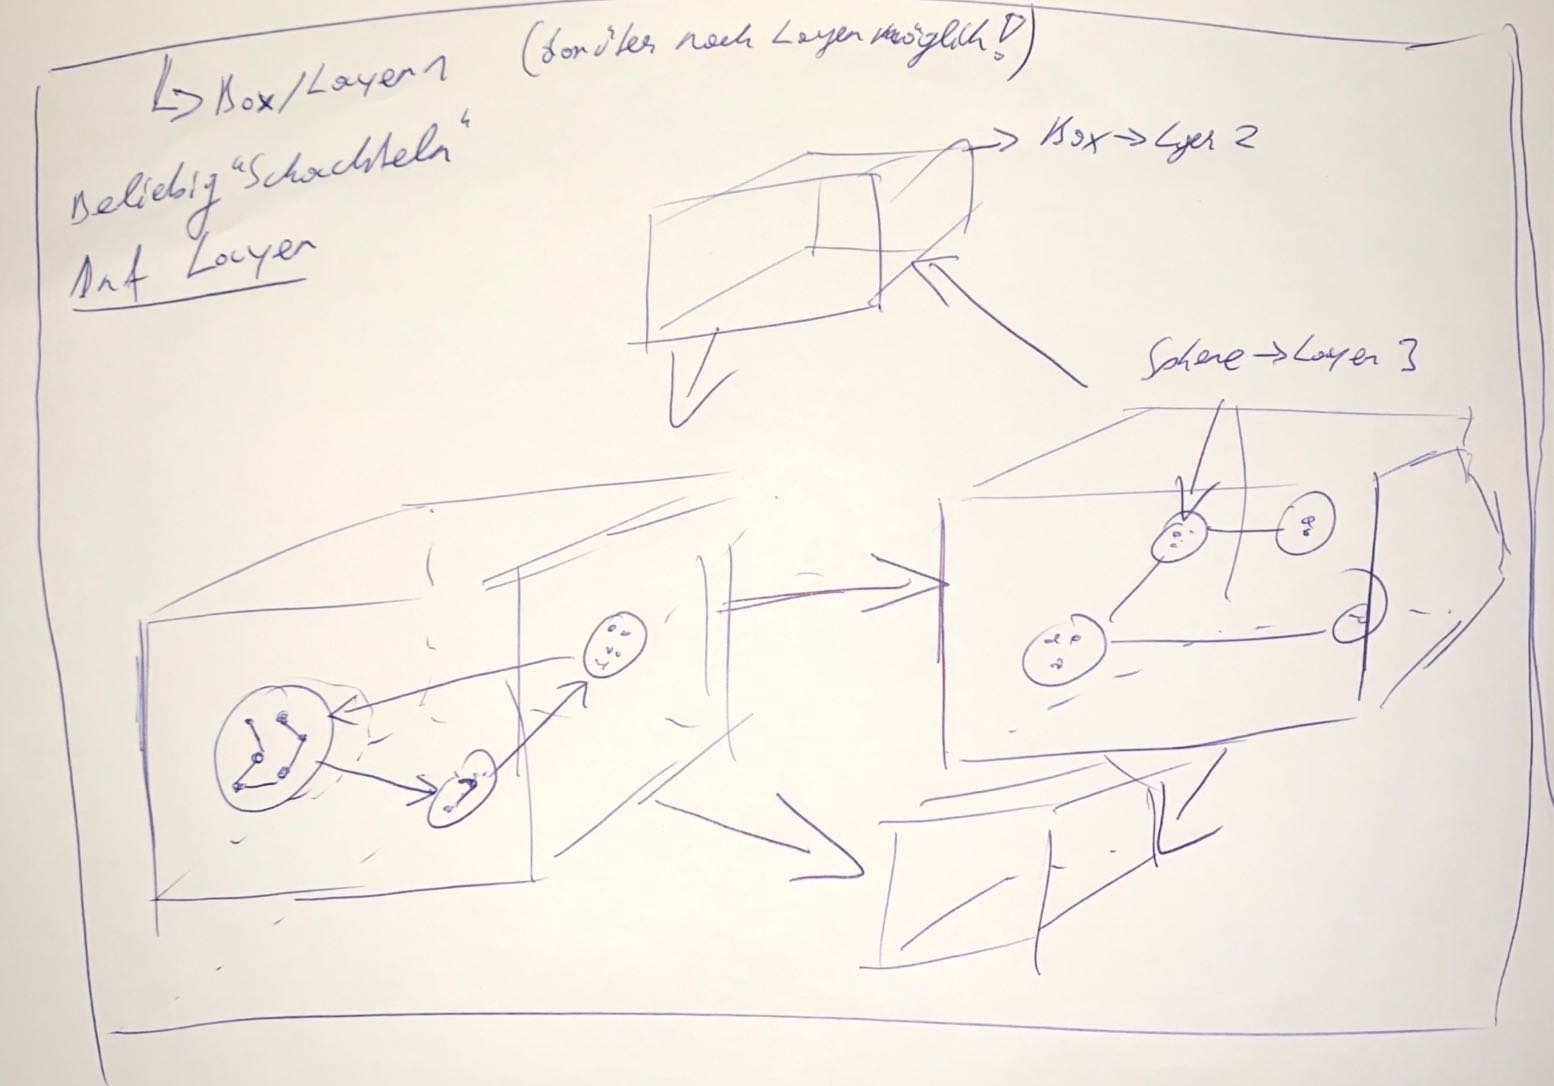
\includegraphics[width=1\textwidth]{chapters/graphics/concept1.jpg}
    \caption{(TODO redraw sketch)A sketch of our preferred layout. } 
    \label{fig:layoutSketch} 
\end{figure}

Figure \ref{fig:layoutSketch} shows a sketch of our layout. The main goal here is to prevent overlapping of nodes while still visualize the different clusters of hierarchical nodes by proximity. The whole data can be seen as a tree structure where each entity in the tree is a graph itself nested in its parent node, therefore the number of nodes grows exponentially with the number of hierarchical layers. Note that the root node is not displayed because it would just create an additional complexity in the visualization without adding any meaningful benefit.
\subsubsection{Layout Forces and Constraints}
We developed a system of multiple forces and constrains to automatically calculate the positions of all nodes. We want to achieve an evenly distributed graph while still fulfilling the rules we set ourselves for hierarchical nesting. Firstly we define a set of force and constraint templates:
\begin{itemize}
    \item ManyBody-Force: This force is a repulsion force and causes nearby nodes to push each other off. The strength decreases with the distance of the nodes. This allows the distribution of nodes evenly among the available space.
    \item Link-Force: It is the counterpart of the ManyBody-Force and pulls nodes connected via a link closer together. Together with the manyBody-Force it enables a distributed graph while clustering connected nodes and minimizing the chance for a link to cross a not involved node.
    \item Collision-Force: This force is basically a reinforces version of the manyBody-Force it prevents nodes from overlapping in the case the manyBody- and Link-Force push nodes into each other.
    \item Spherical-Constraint: The spherical-constraint is the core concept of our layout we use for nesting nodes. It allows us to “squish” multiple nodes in a sphere for any given point and radius. The center of the sphere can variate for each simulation step. The constraint works by constantly adding a slightly randomized velocity for each node towards the center of the sphere, if the node is outside the sphere the velocity is increased drastically.
    \item Center-Force: This force helps us to position the entire visualization in the center of our viewpoint, however there is no strict distance or radius like the spherical-constraint applies.
\end{itemize}

It is important to understand that these templates are not applied equally to all nodes. We apply different entities of forces with different parameters to subsets of our graph. The separation into different subsets allows preventing of interference between different group of nodes for different parents.\\ 
Firstly we distinguish between the top hierarchical layer, from now on called layer $0$, and all other subsequent layers 1,2,3 and so on. Each node and link entity is assigned their respectively layer attribute. Layer $0$ is treated separately because these nodes have no direct assigned parent node. 
For Layer $0$ the center-force with the coordinates $(x:0,y:0,z:0)$, manyBody-force, collision-force and lastly link-force are applied to all nodes and links with layer $0$. 
As for layer $1$ to layer $n$ we not apply forces by layer but instead by parent node. So for each parent we add a collision-force, manyBody-force and link-force for all child nodes and links. In addition, the spherical-constraint is also added for all child nodes with the position of the parent node as a center. Note that the position of the parent node will change each simulation iteration, so we also update the center position for that specific constraint entity.\\
In conclusion, the total number of forces and constraints in our force system is: 
\begin{equation}
    |forces| + |constraints| \: = 4 \, + 4 * |parent\_nodes|
\end{equation}

\subsubsection{Stability of the force system}
(evetuell die gesamte section in einen neuen absatz challenges und raus vom main concept moven)

A big challenge in our force system was to equally balance out all added forces so that each one performs their specific task and does not influence the effect of other forces. To achieve that we parameterized each force with a strength parameter.
In addition to the strength parameter we also use the concept of an alphaTarget from D3.js (cite notwendig?!?). To put it briefly, it is an additional value which decreases throughout the simulation this allows the simulation to “cool down” and stop it as soon as it reaches zero. Besides balancing out the different templates of forces we also have to decrease the strength recursively for each layer as the nodes and their radius get smaller each layer iteration.\\
To improve the stability of the layout we add a small amount of randomness to the applied velocities and strengths, this improves that the nodes are better distributed and prevents strange behavior where multiple nodes are at the exact same location and ruin our force system.\\
During our optimization we stumbled upon the problem that nodes tend to jump rapidly to a far position. This is only natural as we squish the nodes into the sphere of the parent so in some boundary scenarios it is the only way to go for this node. However, it beats up the concept of iteratively fine-tuning the positions throughout the simulation steps, for example nodes of layer 1-3 would be already positioned well but in the last simulation step the parent node in layer 0 would jump and therefore layer 1-3 are position outside the parent layer 0 node again. To circumvent that problem we do not perform the positioning of all nodes throughout the entire simulation, instead we split up the amount of simulation steps and perform them for each layer successively. Luckily we also gain a performance benefit through that strategy as the sum of position update operations reduces essential.
%Verbindung zwischen Datenstruktur und Layout\\
%Ziel des Layouts und Begründung (flexbilität, Kombination standard force based und hierarical/constraint based)\\
%Liste an Forces\\
%Prozess Optimierung der Forces (nacheinander wirken, Sicherheitspuffer)\\
%Wichtigkeit Zusammenhang der Forces mit dem Renderprozess, Stichwort Node Größe
\subsection{Render Visuals}

Wichtigkeit Zusammenhang der Forces mit dem Renderprozess, Stichwort Node Größe\\
Transparente Nodes\\
Node Label + weighted Link\\
different Colors for links\\
Ausblenden des Nodes wenn innerhalb, innersten Node mit Wireframe anzeigen => verbessert Übersichtlichkeit\\

\subsubsection{Exploration Flow}

Grundsätzliche Idee wie die Daten analyisert werden\\
Overview am Beginn => außenansicht \\
Wechsel zur Detailansicht\\
Möglichkeit von Room scale voll ausschöpfen, walk around the vis\\
Verschiedene Filteroptionen für Edges (nur grundidee)\\
Verschiedene Navigationsmethoden (nur grundidee)\\

\section{Navigation + Interaction}

Laserpointer Interaktion zum selektieren von Nodes / links\\
Navigations Methoden\\
Anzeige des currentLayers am Controller\\
Grafik mit Controller button belegung\\

\section{Challenges}

Visual Clutter: Filtermethoden von links (2 separated methods)\\

Problem Größenbezug real world + virtual scene\\
1. Dynamischen fly speed\\
2. Dynamisches skalieren\\
manueller speed + skalierung wichtig da nicht klar was User preferred und wie groß sein space ist\\ 


\section{(eventuell) Alternative Concepts}

verworfene Konzepte, 2 Layer Concept\\

\chapter{old - Proposed Solution}
Ideas:
\begin{itemize}
    \item Progress
        \begin{itemize}
            \item begin flat multilayer rendering
        \end{itemize}
\end{itemize}

\section{Concepts}
\subsection{Original 2D Visualization}
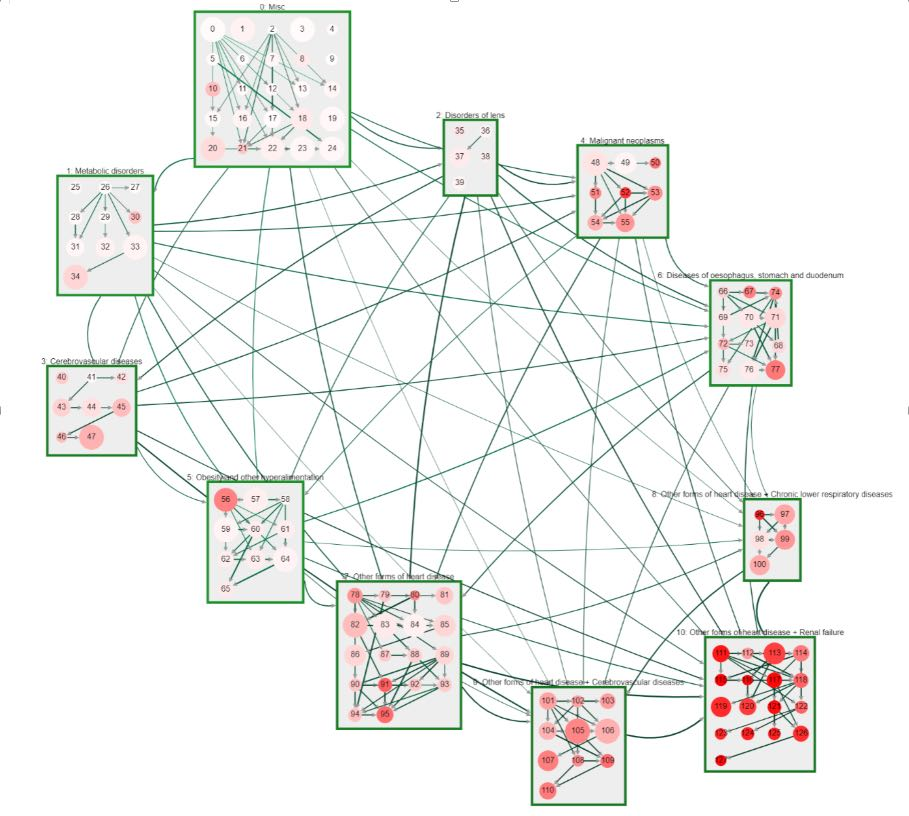
\includegraphics[width=0.5\textwidth]{chapters/graphics/2dVisOfDemoData.jpg}

Problem only two layers supported

\subsection{2-Layer Concept}
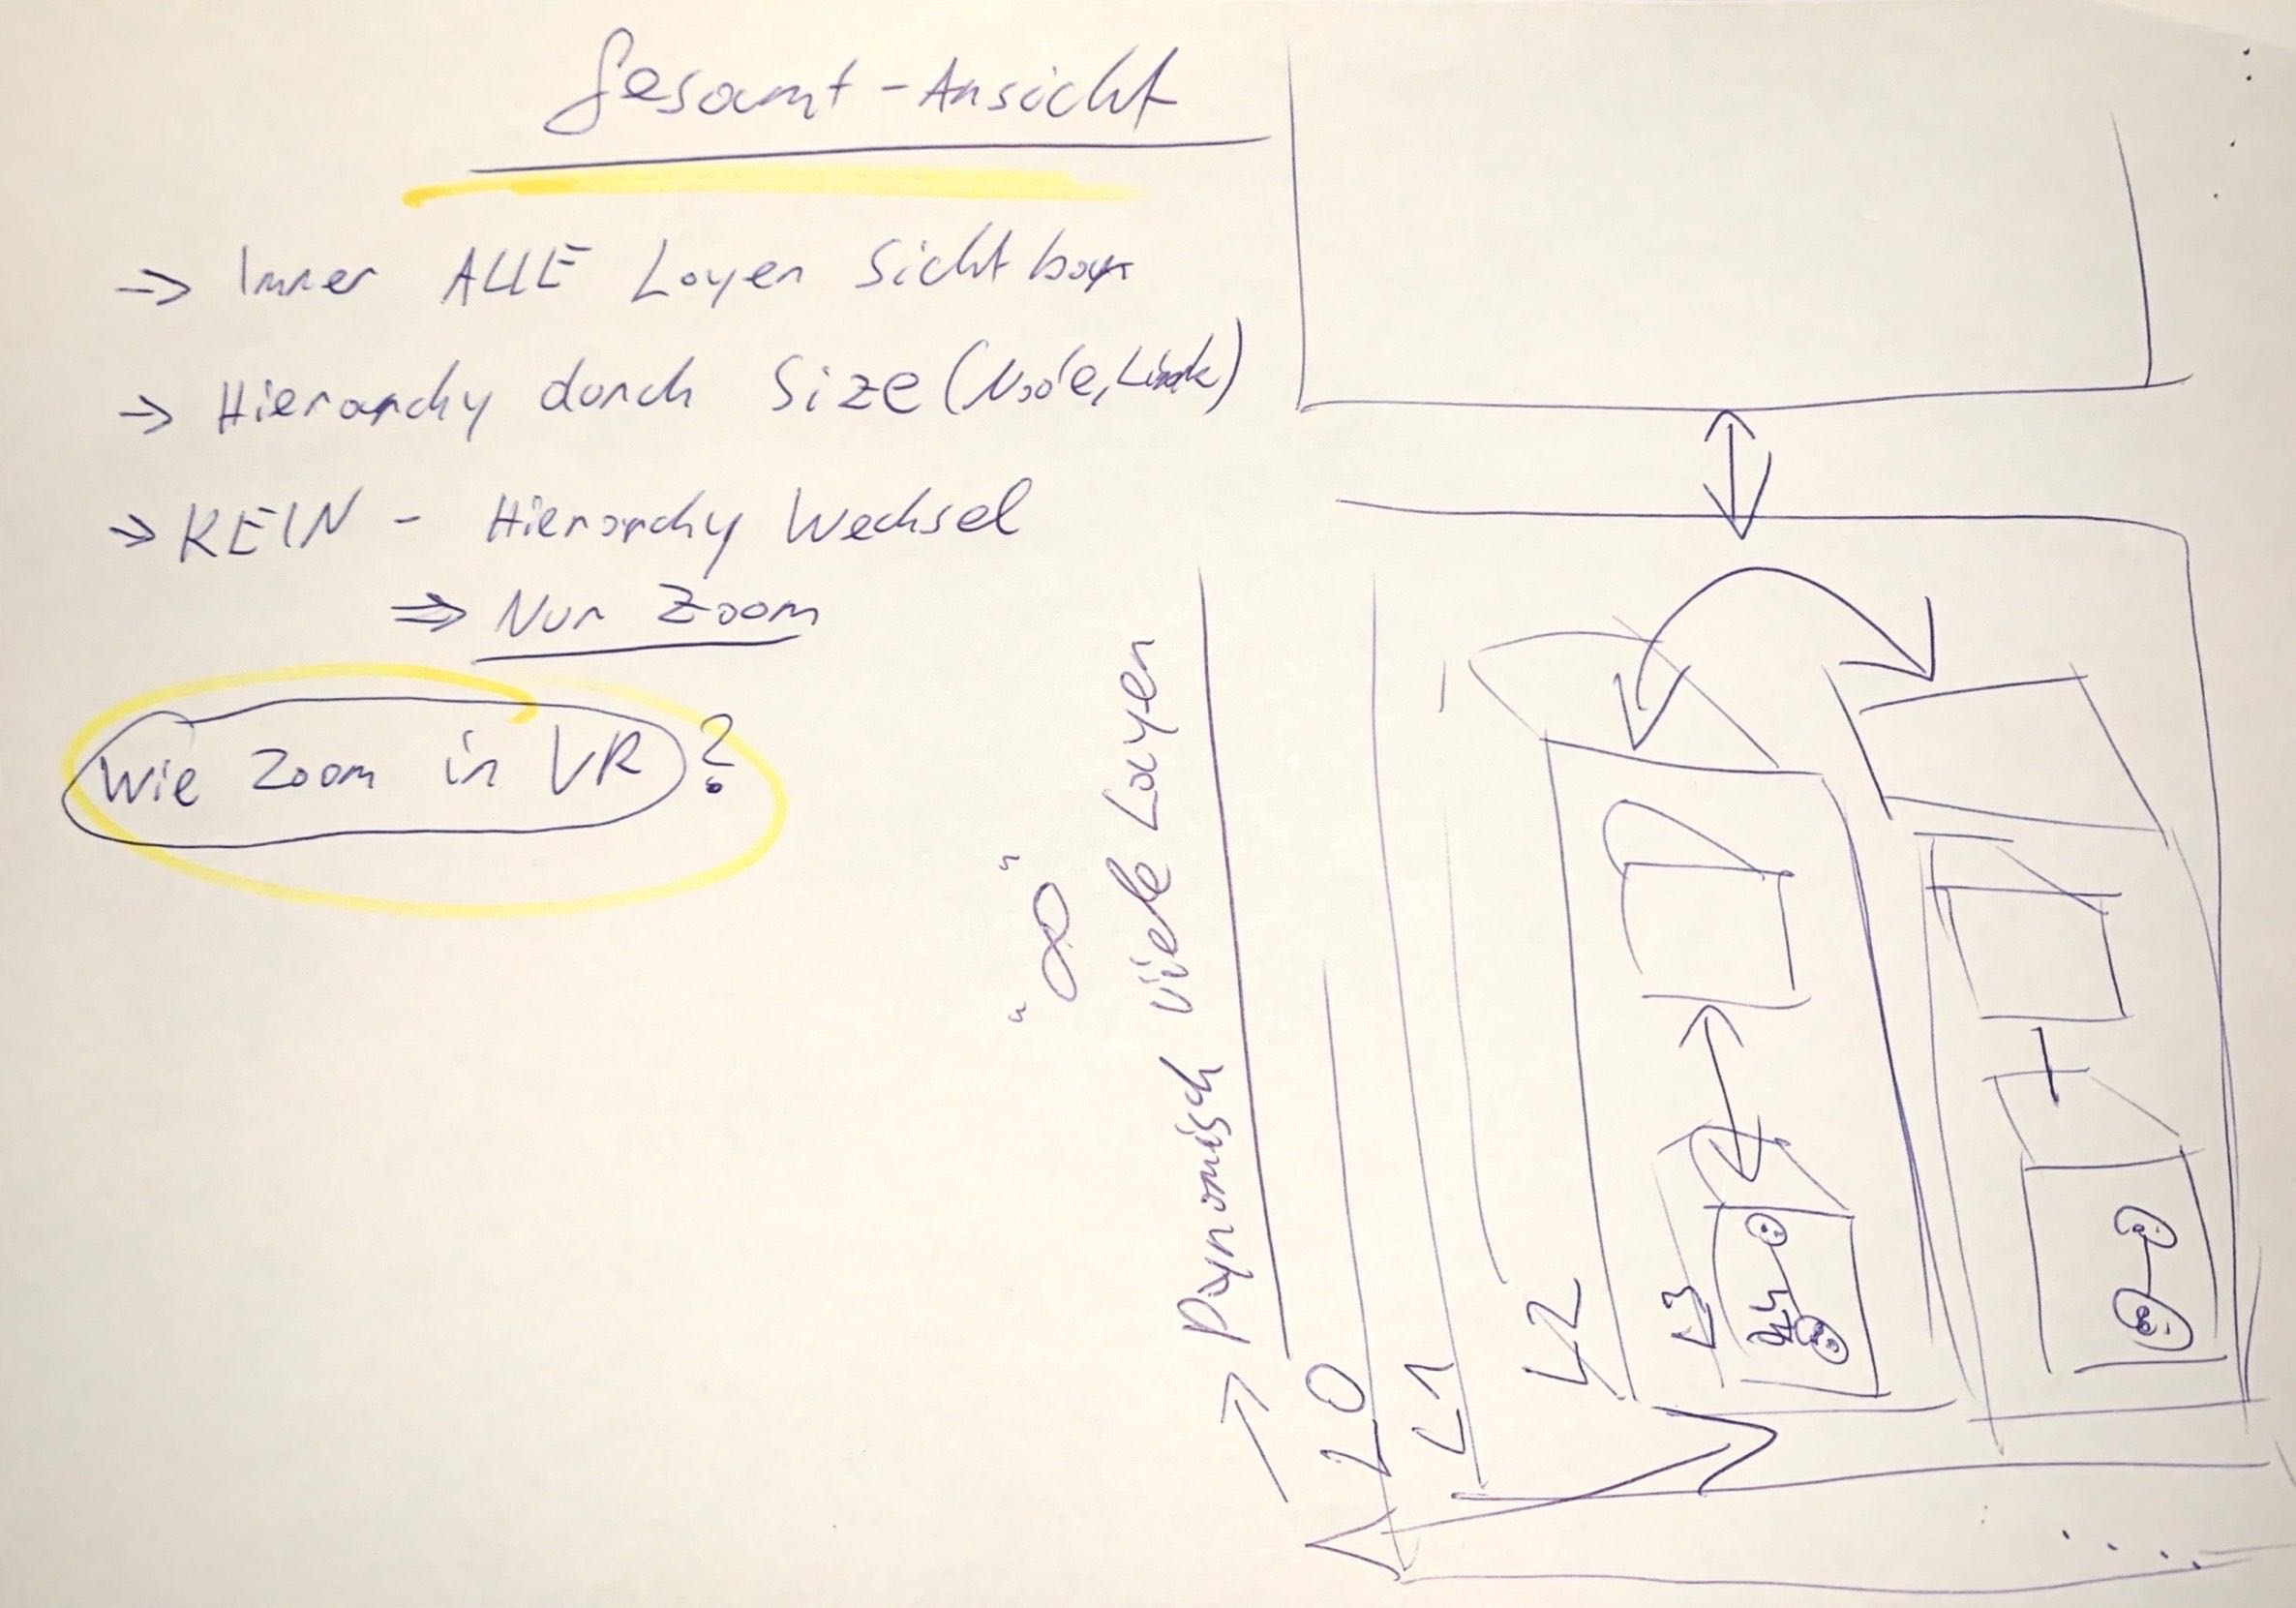
\includegraphics[width=0.5\textwidth]{chapters/graphics/concept2.jpg}

Cube/ (half) sphere position of sub-graphs \\
Starting idea, why it was discarded

\subsection{n-Layer Concept}
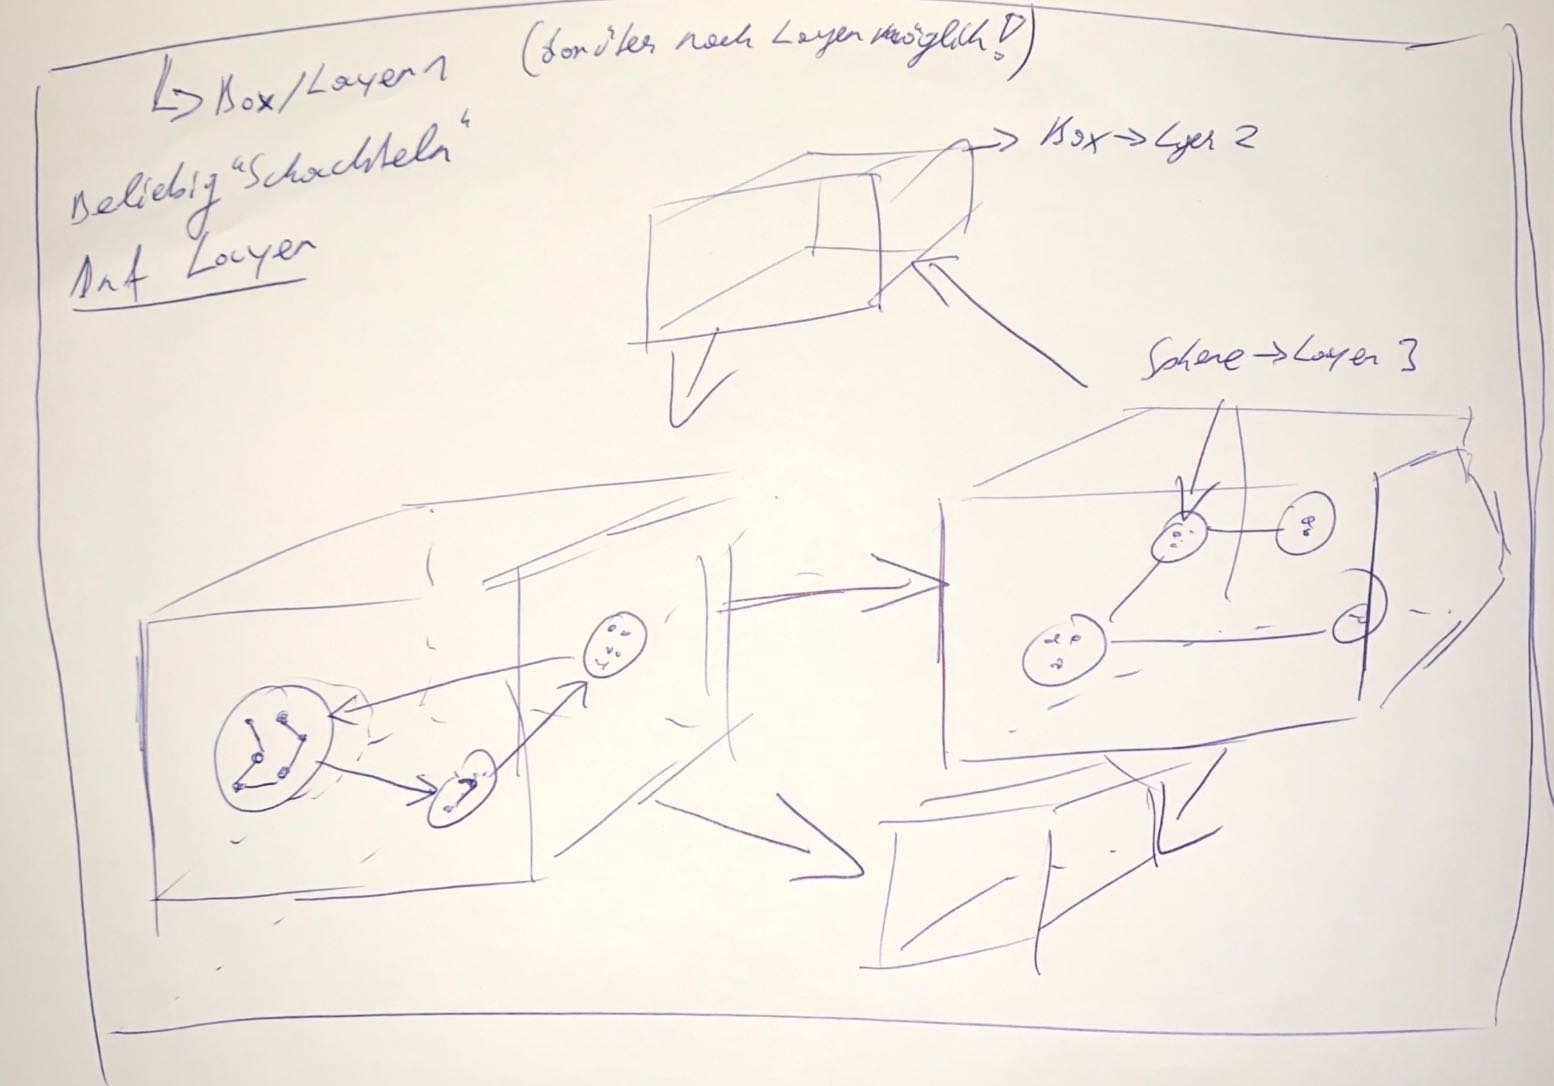
\includegraphics[width=0.5\textwidth]{chapters/graphics/concept1.jpg}

Improved concept \\
no fixed cube/(half) sphere position instead each layer calculate its own position \\
circle over boxes \\
Begin: flyspeed only, later on problem on VR \\

\section{Position of Nodes}

Independent per layer / sub-graph inside parent node \\
use of existing implemented and already good tested(prevents overlapping, good distribution, ...) forces (collision, link, manyBody, ...) \\
use of own forces to place sub-graphs inside parent graphs \\
adjustable force strengths \\
Node size grow with number of child nodes \\
\\
two possible solutions: web-worker vs live \\

\section{Usage of different Visual Features}

Position \\
linkWidth \\
linkColor \\
linkDirection \\ 
currentLayer on Controller Overlay \\ 

\section{Graph Exploration}

\subsection{Overview Layout}
Orbital Camera

\subsection{Detail Layout}
Free Fly Camera \\
change FlySpeed based on current node the camera is located. As deeper the layer as slower the flyspeed \\
Problem experiments showed this does not work well in VR --> manual / automated scaling. \\

flyToNode \\
flyToParentLayer \\

\subsection{Visibility of the Visualization}
\subsubsection{Nodes / Layers}
wireframe
\subsubsection{Links}
lockLinks

\section{Interaction}
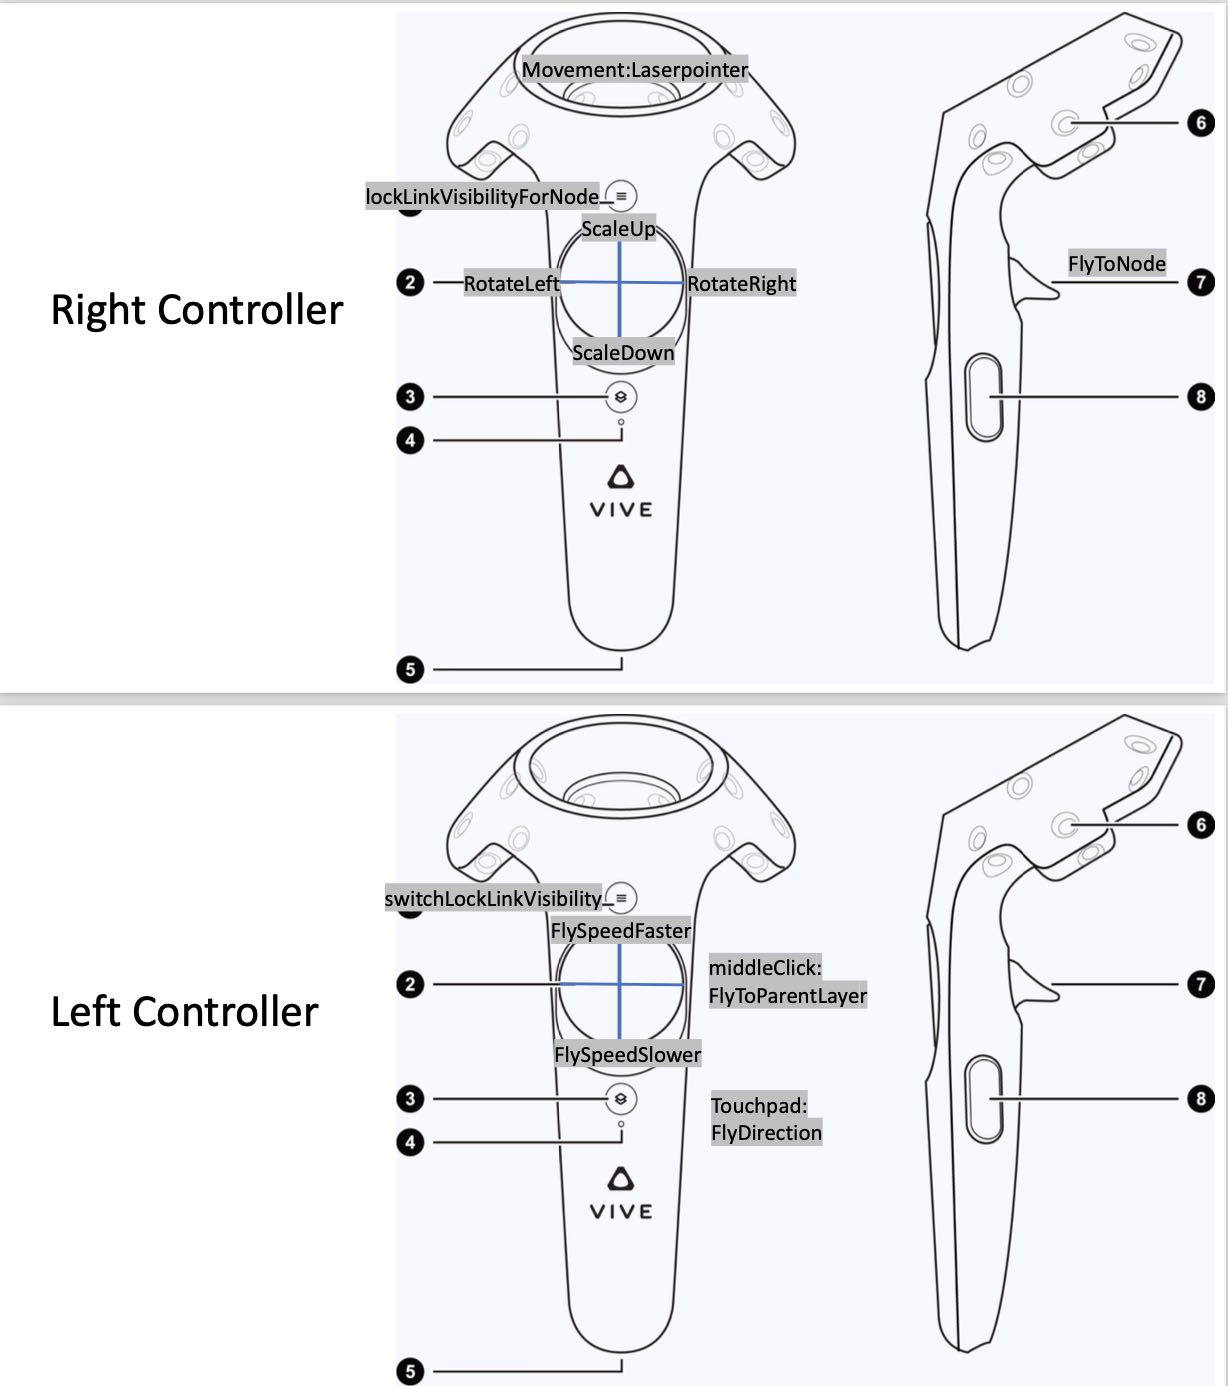
\includegraphics[width=0.5\textwidth]{chapters/graphics/controllerMapping.jpg}
